 
\documentclass[conference]{IEEEtran}
%\IEEEoverridecommandlockouts
% The preceding line is only needed to identify funding in the first footnote. If that is unneeded, please comment it out.
\usepackage{cite}
\usepackage[ngerman]{babel}
\usepackage[utf8]{inputenc}
\usepackage{amsmath,amssymb,amsfonts}
\usepackage{algorithmic}
\usepackage{float}
\usepackage{graphicx}
\usepackage{textcomp}
\usepackage{xcolor}
\usepackage{listings}

\bibliographystyle{ieeetr}


\definecolor{pblue}{rgb}{0.13,0.13,1}
\definecolor{pgreen}{rgb}{0,0.5,0}
\definecolor{pred}{rgb}{0.9,0,0}
\definecolor{pgrey}{rgb}{0.46,0.45,0.48}
\lstset{language=Java,
	showspaces=false,
	showtabs=false,
	breaklines=true,
	tabsize=2,
	showstringspaces=false,
	breakatwhitespace=true,
	commentstyle=\color{pgreen},
	keywordstyle=\color{pblue},
	stringstyle=\color{pred},
	basicstyle=\ttfamily
}


\usepackage{url}
\def\BibTeX{{\rm B\kern-.05em{\sc i\kern-.025em b}\kern-.08em
    T\kern-.1667em\lower.7ex\hbox{E}\kern-.125emX}}
\begin{document}

\title{Medizinische Bildverarbeitung - Lab 2}

\author{\IEEEauthorblockN{Eldin Ramic, Alexander Straube}
\IEEEauthorblockA{\textit{Hochschule München} \\
München, Deutschland \\
ramic@hm.edu, straube@hm.edu}
}

\maketitle

\section{Aufgabenstellung}
Im zweiten Laboratorium war das Ziel einen DICOM (Digital Imaging and Communications in Medicine) Volumenbilddatensatz einzulesen, zu verarbeiten und auf unterschiedlicher Art darzustellen.

Zuerst soll ein einzelner Schnitt (Slice) des Datensatzes dargestellt werden, wonach der komplette generierte Volumendatensatz als Gittermodell (Wireframe) angezeigt werden soll. Hierbei ist der Detailgrad des Gittermodells zu hoch und kostet viel Performance, sodass das Deteillevel der Daten zu reduzieren ist.

In der vierten Aufgabe soll der Datensatz mit einer Oberfläche dargestellt und entsprechend beleuchtet werden.

Zuletzt soll der Halterungskäfig aus den Bilddaten entfernt werden, sodass nur noch die Maus zu sehen ist.

\section{Volumenbilddatensatz}

Der gegebene Datensatz umfasst 385 DICOM Dateien, die jeweils Daten, wie das Pixel Array, das Pixel Spacing, Image Position Patient oder andere Header und Meta Informationen, enthalten.

Das Pixel Array ist ein Numpy Array und enthält die Pixel Daten des CT Bildes im Hounsfiled Format. Mit der Hounsfield-Skala wird in der Computertompgraphie (CT) die Abschwächung von Röntgenstrahlung in Gewebe beschrieben und in Graustufenbildern dargestllt. \cite{wiki:HU} \\
Das Pixel Spacing ist der physikalische Abstand im Patienten zwischen der Mitte jedes Pixels, angegeben durch ein numerisches Paar. Diese Information ist wichtig für die Darstellung des Datensatz in einem 3D Gittermodell. \\
Das Image Position Patient Attribut gibt die Bildposition im 3 dimensionalem Raum an. Die x-, y- und z-Koordinaten geben den Mittelpunkt des ersten übertragenen Voxels in der linken oberen Ecke des Bildes an.\cite{pixel_spacing} \\

Mithilfe von Matplotlib haben wir ein Histogramm erstellt\ref{slice_hist}, welches die Häufigkeit von bestimmten Hounsfield Units (HU) in allen Bildern des Volumendatensatzes in Relation setzt. \\

\begin{tabular}{|c|c|c|c|c|}		
		\hline
		\textbf{Substanz} & \textbf{HU} & \textbf{--} & \textbf{Substanz} & \textbf{HU}\\
		\hline
		Luft & -1000 & -- & Muskeln & +40\\
		\hline
		Fett & -120 & -- & Kontrast & +130\\
		\hline
		Wasser & 0 & -- & Knochen & +400\\
		\hline
	\end{tabular}\\


Das Histogramm verdeutlicht, dass Pixel mit einem HU von -1000 am Häufigsten vorkommen, was die Substanz Luft repräsentiert. Die Tabelle zeigt die verschiedenen Substanzen, die durch HU definiert werden.

\begin{figure}[H]
	\begin{center}
		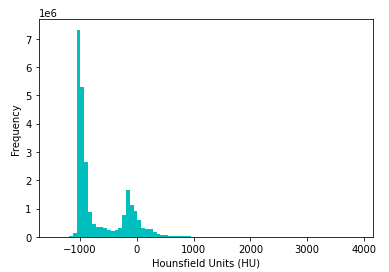
\includegraphics[width=6.5cm]{latex/images/slices_hist.png}
	 	\caption{Häufigkeit von HU aller Bilddaten}
	 	\label{slice_hist}
	\end{center}
\end{figure}

\section{Einlesen der Daten}
Im ersten Schritt sollen die DICOM Daten aus dem Data-Verzeichnis eingelesen und in entsprechenden Datnestrukturen gespeichert werden.

Mithilfe des Pydicom Python Package\cite{pydicom} können über den Pfad des Data-Verzeichnis alle DICOM Dateien eingelesen, und in einer Liste von FileDatasets gespeichert werden. Dabei wird die Acquisition Number aus den Header Informationen verwendet, um die Schnittbilder in die richtige Reihenfolge zu bringen. \\
Bei der Erstellung einer eigenen Liste mit allen Numpy Arrays, werden die Bilder zusätzlich um 180° gedreht, da ein Fehler bei der Erstellung des Volumendatensatzes auftrat.

\section{Visualisierung der Schnittbilder}
Abbildung \ref{slices} zeigt das Schnittbild an der 150. Stelle im Bilddatensatz auf der linken Seite mit der Colormap "bone" und auf der rechten Seite mit der Colormap "gray".

\begin{figure}[H]
	\begin{center}
		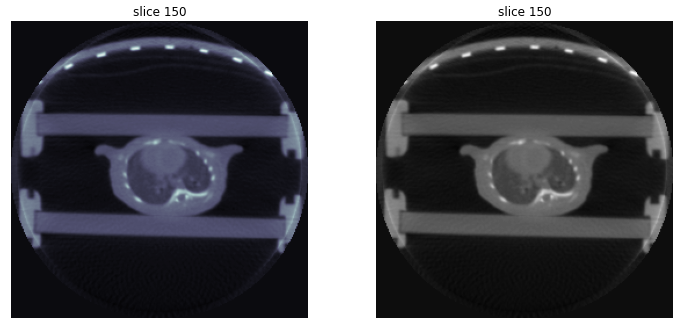
\includegraphics[width=6.5cm]{latex/images/slice_150.png}
	 	\caption{150. Schnittbild des Volumendatensatzes}
	 	\label{slice_150}
	\end{center}
\end{figure}

Abbildung \ref{slices} zeigt neun weitere Schnittbilder des Datensatzes, sodass man eine 3 dimensionale Abbildung einer Maus antizipieren kann.

\begin{figure}[H]
	\begin{center}
		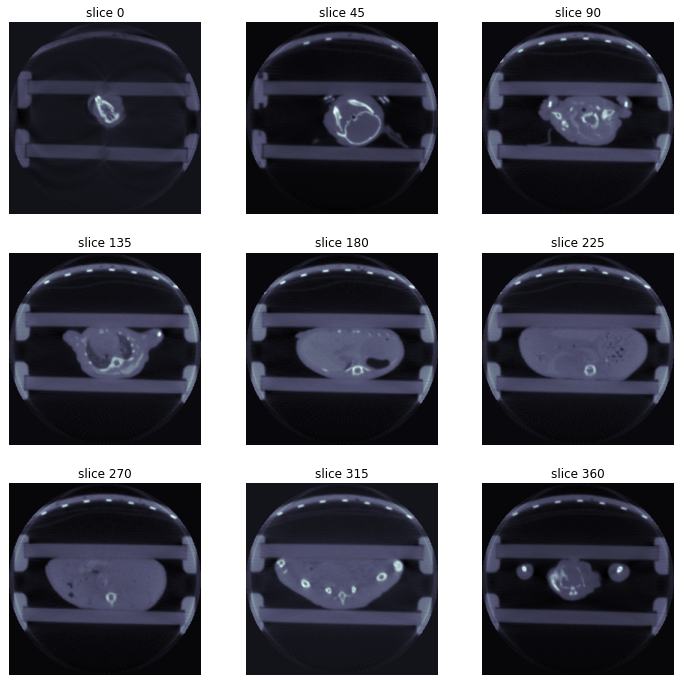
\includegraphics[width=8cm]{latex/images/slices.png}
	 	\caption{weitere Schnittbilder des Volumendatensatzes}
	 	\label{slices}
	\end{center}
\end{figure}

Zusätzlich haben wir eine interaktive Plot Methode implementiert, bei der man über eine Slide-Bar alle Bilder hintereinander anschauen kann. Der zugehörige Code befindet sich im Repository als dicom\_animation Methode.

\section{Darstellen des Volumendatensatzes als Wireframe}
In der dritten Aufgabe ist es das Ziel den Volumendatensatz als Gittermodell anzeigen zu lassen. Dafür gibt es in Python verschiedene Herangehensweisen und Bibliotheken, die auch ein interaktives Gittermodell ermöglichen.

\subsection{Darstellen des Volumendatensatzes mit Beleuchtung und Oberfläche}

\section{Entfernung des Halterungskäfigs aus den Bilddaten}

\section{Programmiersprache, Programm Architektur, Entwicklungsumgebung}
 
\section{Evaluierung der Ergebnisse}
	
	Vielleicht noch bisle mehr Evaluieren?


\section{Polygon Unit Tests}


\section{Anhang}


\bibliography{literature}

\end{document}